\begin{frame}{Experiments}
\textbf{Datasets: }
    \begin{enumerate}
        \item Wikipedia articles (\abr{en}, \abr{zh})
        \item Amazon reviews (\abr{en}, \abr{zh}) 
        \item \abr{lorelei} documents (\abr{en}, \abr{si})
    \end{enumerate} 
\end{frame}

\begin{frame}{Experiments}
\textbf{Metrics: }
    \begin{enumerate}
        \item Classification accuracy
        \begin{itemize}
            \item Intra-lingual: train topic model on documents in one language and test on other documents in the \emph{same} languages
            \item Cross-lingual: train topic model on documents in one language and test on other documents in a \emph{different} language.
        \end{itemize}
        \item Topic coherence~\citep{lau-2014}.
        \begin{itemize}
            \item Intrinsic: use the trained documents as the reference corpus to measure local interpretability.
            \item Extrinsic: use a large dataset (i.e. entire Wikipedia) as the reference corpus to measure global interpretability. 
        \end{itemize}
    \end{enumerate}
\end{frame}

\begin{frame}{Comparing Models}
\begin{table}
  \centering
  \scriptsize
  \begin{tabular}{llllll} \\
    & & \multicolumn{4}{c}{Classification accuracy} \\
    \cmidrule(r){3-6} 
    Dataset & Method & \abr{en-i} & \makecell{\abr{zh-i}\\\abr{si-i}} & \abr{en-c} & \makecell{\abr{zh-c}\\\abr{si-c}} \\
    \midrule 
    Wikipedia & \makecell{Multilingual\\anchoring} & 69.5\% & 71.2\% & 50.4\% & 47.8\% \\
    & \makecell{\mtanchor\\(maximum)} & \textbf{80.7}\% & \textbf{75.3}\% & \textbf{57.6}\% & \textbf{54.5}\% \\
    & \makecell{\mtanchor\\(median)} & 69.5\% & 71.4\% & 50.3\% & 47.2\% \\
    & \abr{mcta} & 51.6\% & 33.4\% & 23.2\% & 39.8\%  \\
    \midrule
    Amazon & \makecell{Multilingual\\anchoring} & \textbf{59.8}\% & \textbf{61.1}\% & \textbf{51.7}\% & \textbf{53.2}\% \\
    & \abr{mcta} & 49.5\% & 50.6\% & 50.3\% & 49.5\% \\
    \midrule 
    \abr{lorelei} & \makecell{Multilingual\\anchoring} & \textbf{20.8}\% & \textbf{32.7}\% & \textbf{24.5}\% & \textbf{24.7}\% \\
    & \abr{mcta} & 13.0\% & 26.5\% & 4.1\% & 15.6\%  \\
  \end{tabular}
\end{table}
\end{frame}


\begin{frame}{Comparing Models}
\begin{table}
  \centering
  \scriptsize
  \begin{tabular}{llllllllll} \\
    & & \multicolumn{4}{c}{Topic coherence} \\
    \cmidrule(r){3-6}
    Dataset & Method & \abr{en-i} & \makecell{\abr{zh-i}\\\abr{si-i}} & \abr{en-e} & \makecell{\abr{zh-e}\\\abr{si-e}} \\
    \midrule 
    Wikipedia & \makecell{Multilingual\\anchoring} & 0.14 & 0.18 & 0.08 & 0.13  \\
    & \makecell{\mtanchor\\(maximum)} & \textbf{0.20} & \textbf{0.20} & \textbf{0.10} & \textbf{0.15} \\
    & \makecell{\mtanchor\\(median)} & 0.14 & 0.18 & 0.08 & 0.13\\
    & \abr{mcta} & 0.13 & 0.09 & 0.00 & 0.04  \\
    \midrule
    Amazon & \makecell{Multilingual\\anchoring} & \textbf{0.07} & \textbf{0.06} & \textbf{0.03} & \textbf{0.05} \\
    & \abr{mcta} & -0.03 & 0.02 & 0.02 & 0.01 \\
    \midrule 
    \abr{lorelei} & \makecell{Multilingual\\anchoring} & 0.08 & 0.00 & 0.03 & n/a \\
    & \abr{mcta} & \textbf{0.13} & 0.00 & \textbf{0.04} & n/a  \\
  \end{tabular}
\end{table}
\end{frame}

\begin{frame}{Multilingual Anchoring Is Much Faster}
\begin{figure}
\begin{overprint}
\centerline{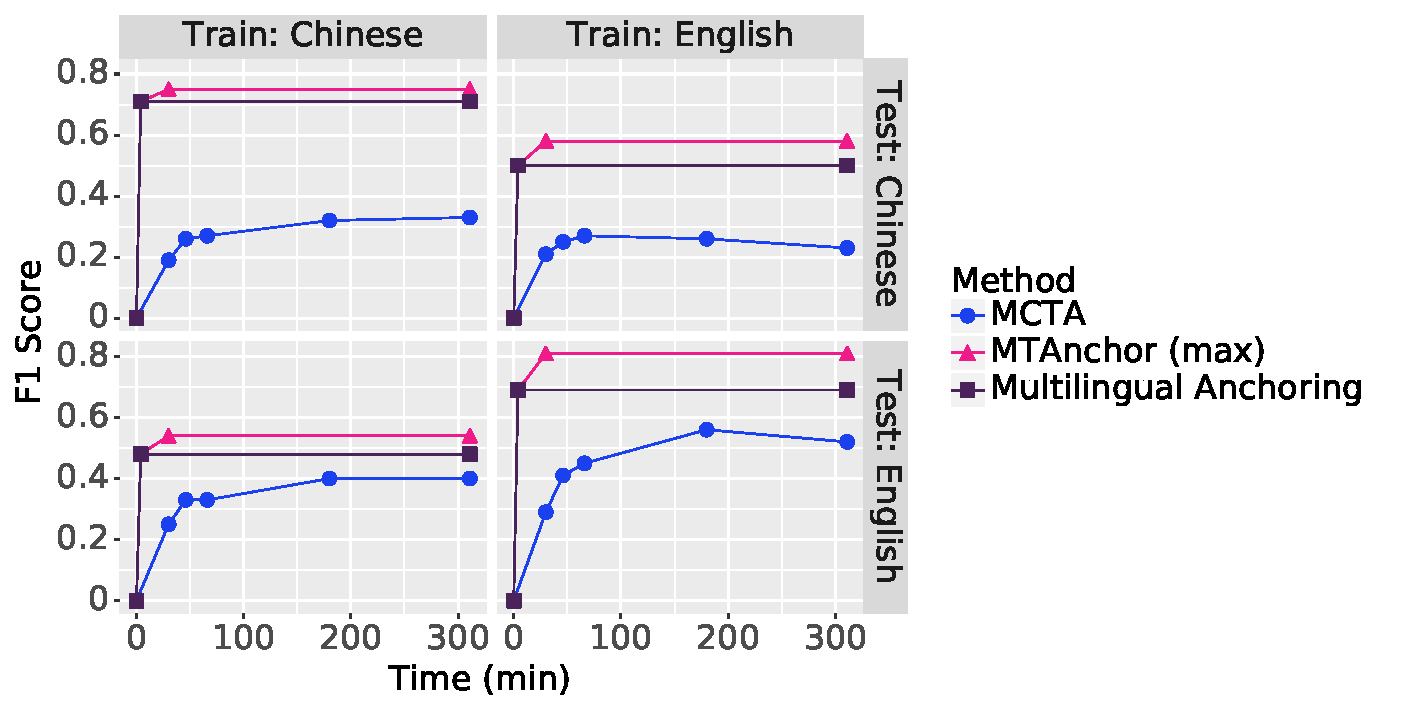
\includegraphics[width=0.9\textwidth]{methods_wiki.pdf}}
\end{overprint}
\end{figure}
\end{frame}

\begin{frame}{Improving Topics Through Interactivity}
\begin{figure}
\begin{overprint}
\onslide<1> \centerline{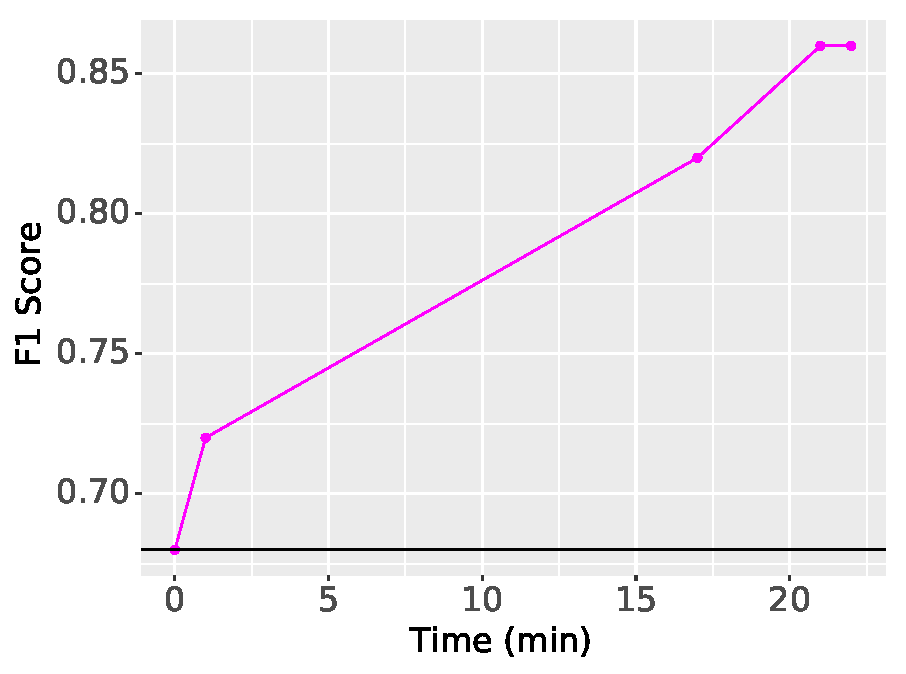
\includegraphics[width=0.9\textwidth]{user_exp1.pdf}}
\onslide<2> \centerline{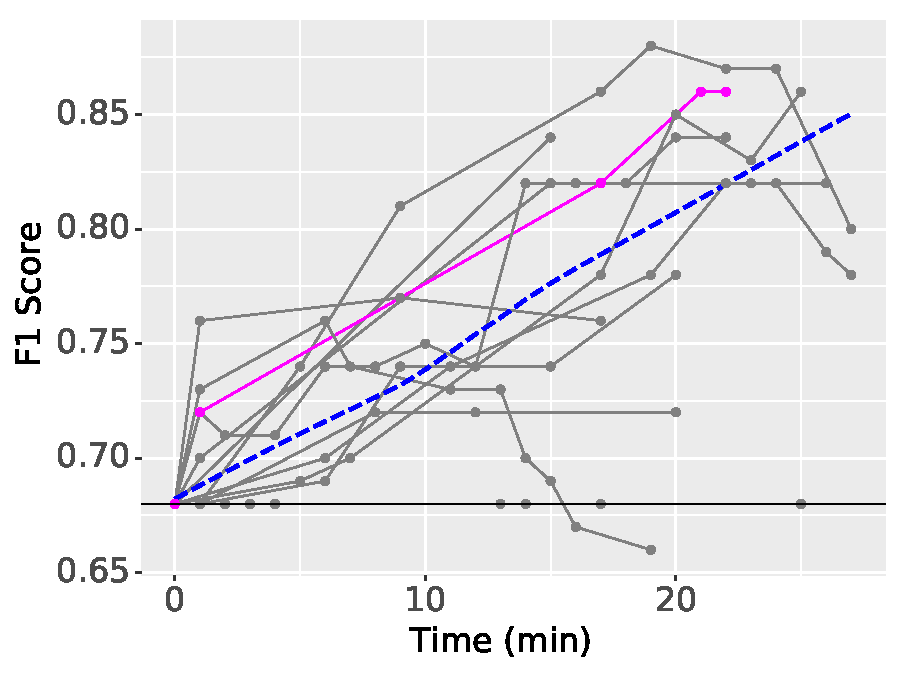
\includegraphics[width=0.9\textwidth]{user_exp2.pdf}}
\onslide<3-> \centerline{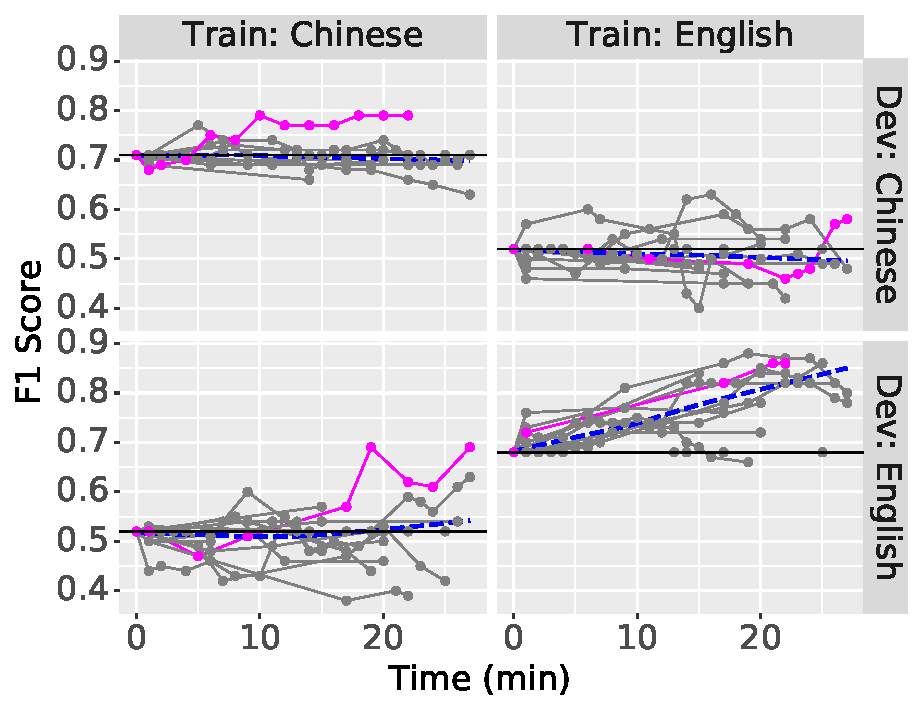
\includegraphics[width=0.9\textwidth]{user_exp3.pdf}}
\end{overprint}
\end{figure}
\end{frame}

